\documentclass[aspectratio=169]{beamer}
\usetheme{Madrid}
\usecolortheme{default}

% Packages
\usepackage[utf8]{inputenc}
\usepackage{graphicx}
\usepackage{listings}
\usepackage{xcolor}
\usepackage{tikz}
\usepackage{hyperref}
\usetikzlibrary{shapes.geometric, arrows, positioning, calc}

% Code listing style
\lstset{
    basicstyle=\ttfamily\footnotesize,
    keywordstyle=\color{blue},
    commentstyle=\color{green!60!black},
    stringstyle=\color{red},
    breaklines=true,
    frame=single,
    numbers=left,
    numberstyle=\tiny\color{gray}
}

% TikZ styles
\tikzstyle{agent} = [rectangle, rounded corners, minimum width=2.5cm, minimum height=1cm, text centered, draw=black, fill=blue!20]
\tikzstyle{process} = [rectangle, minimum width=2.5cm, minimum height=1cm, text centered, draw=black, fill=orange!20]
\tikzstyle{arrow} = [thick,->,>=stealth]

% Title page information
\title[Dual-Agent Debate System]{Dual-Agent Debate Matchmaking System\\Based on Similarity and Diversity Strategies}
\author{
    Jyoti Triklani AU2544015\\
    Gautam Prajapati AU2544033
}
\institute[Ahmedabad University]{
    Department - Masters in Computer Science & Engineering \\
    School of Engineering And Science (SEAS)\\
    Ahmedabad University
}
\date{21st November 2025}

\begin{document}

% Slide 1: Title
\begin{frame}
    \titlepage
    \centering
    \small Course: CSE601 Computational Thinking\\
    \small Instructor: Dr. Shristi Sharma
\end{frame}

% Slide 2: Table of Contents
\begin{frame}{Outline}
    \tableofcontents
\end{frame}

% Slide 3: Introduction & Problem
\section{Problem Statement}
\begin{frame}{Problem Statement}
    \begin{block}{Challenges in Current Debate Systems}
        \begin{itemize}
            \item Online debate platforms often produce mismatched opponents
            \item Leads to unengaging or unbalanced discussions
            \item Single-agent algorithms fail to capture full range of perspectives
            \item Users experience frustration with poor debate pairings
        \end{itemize}
    \end{block}
    
    \vspace{0.3cm}
    
    \begin{block}{Need for AI-Driven Solution}
        \begin{itemize}
            \item Dynamic matching strategies required
            \item Combination of similarity and diversity approaches
            \item Multi-agent system for balanced arguments
            \item Automated evaluation for fair judgment
        \end{itemize}
    \end{block}
\end{frame}

% Slide 4: Solution Overview
\section{Solution Overview}
\begin{frame}{Our Solution: Dual-Agent System}
    \begin{columns}
        \begin{column}{0.48\textwidth}
            \textbf{System Components:}
            \begin{itemize}
                \item \textbf{Agent Alpha:} Logical arguments
                \item \textbf{Agent Beta:} Emotional arguments
                \item \textbf{Moderator:} Automated judgment
                \item \textbf{Gemini API:} LLM backend
                \item \textbf{LangGraph:} Orchestration
            \end{itemize}
            
            \vspace{0.4cm}
            
            \textbf{Key Features:}
            \begin{itemize}
                \item Automatic position assignment
                \item Multi-round debates
                \item Fair scoring mechanism
            \end{itemize}
        \end{column}
        
        \begin{column}{0.48\textwidth}
            \begin{center}
                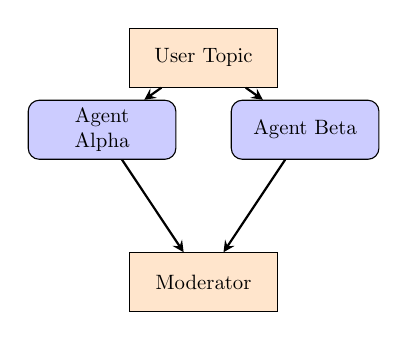
\begin{tikzpicture}[node distance=1.3cm, scale=0.75, transform shape]
                    \node (user) [process, text width=2cm] {User Topic};
                    \node (agent1) [agent, below left of=user, xshift=-0.8cm, yshift=-0.3cm, text width=1.8cm] {Agent Alpha};
                    \node (agent2) [agent, below right of=user, xshift=0.8cm, yshift=-0.3cm, text width=1.8cm] {Agent Beta};
                    \node (mod) [process, below of=user, yshift=-2.5cm, text width=2cm] {Moderator};
                    
                    \draw [arrow] (user) -- (agent1);
                    \draw [arrow] (user) -- (agent2);
                    \draw [arrow] (agent1) -- (mod);
                    \draw [arrow] (agent2) -- (mod);
                \end{tikzpicture}
            \end{center}
            \vspace{0.2cm}
            \centering
            \footnotesize \textit{Figure: System Architecture}
        \end{column}
    \end{columns}
\end{frame}

% Slide 5: Literature Review
\section{Literature Review}
\begin{frame}{Literature Review}
    \begin{block}{Foundational Research}
        \begin{itemize}
            \footnotesize
            \item \textbf{Multi-Agent Systems} \cite{wooldridge1995}
            \begin{itemize}
                \scriptsize
                \item Wooldridge \& Jennings (1995): Theory and practice of intelligent agents
                \item Foundation for autonomous agent collaboration and competition
            \end{itemize}
            
            \item \textbf{Computational Thinking} \cite{wing2006}
            \begin{itemize}
                \scriptsize
                \item Wing (2006): Foundational framework for problem-solving
                \item Four pillars: Decomposition, Pattern Recognition, Abstraction, Algorithms
            \end{itemize}
        \end{itemize}
    \end{block}
    
    \begin{block}{Modern AI Technologies}
        \begin{itemize}
            \footnotesize
            \item \textbf{Transformer Architecture \& LLMs} \cite{vaswani2017, brown2020}
            \begin{itemize}
                \scriptsize
                \item Vaswani et al. (2017): Attention mechanism for NLP
                \item Brown et al. (2020): GPT-3 few-shot learning capabilities
            \end{itemize}
            
            \item \textbf{Implementation Tools} \cite{langgraph2024, gemini2024, streamlit2024}
            \begin{itemize}
                \scriptsize
                \item LangGraph: Multi-agent workflow orchestration
                \item Google Gemini API: Advanced language model
                \item Streamlit: Interactive web interfaces
            \end{itemize}
        \end{itemize}
    \end{block}
\end{frame}

% Slide 6: Decomposition & Pattern Recognition
\section{Computational Thinking Framework}
\begin{frame}{CT Pillar 1 \& 2: Decomposition and Pattern Recognition}
    \begin{columns}[t]
        \begin{column}{0.48\textwidth}
            \begin{block}{1. Decomposition}
                \textbf{System broken into modules:}
                \begin{itemize}
                    \item Input Processing Module
                    \item Agent Management (Pro, Con, Judge)
                    \item Gemini API Integration
                    \item Argument Generation Engine
                    \item Scoring \& Evaluation System
                    \item Results Display Module
                \end{itemize}
            \end{block}
        \end{column}
        
        \begin{column}{0.48\textwidth}
            \begin{block}{2. Pattern Recognition}
                \textbf{Identified patterns:}
                \begin{itemize}
                    \item \textbf{Argument Structure:}\\
                    Claim $\rightarrow$ Evidence $\rightarrow$ Reasoning
                    \item \textbf{Debate Flow:}\\
                    Opening $\rightarrow$ Rebuttals $\rightarrow$ Closing
                    \item \textbf{Evaluation Criteria:}\\
                    Logic, Evidence, Relevance, Persuasiveness
                    \item API response parsing patterns
                \end{itemize}
            \end{block}
        \end{column}
    \end{columns}
\end{frame}

% Slide 6: Abstraction & Algorithm Design
\begin{frame}{CT Pillar 3 \& 4: Abstraction and Algorithm Design}
    \begin{columns}[t]
        \begin{column}{0.48\textwidth}
            \begin{block}{3. Abstraction}
                \textbf{Hiding complexity:}
                \begin{itemize}
                    \item Agent behavior unified across all topics
                    \item API complexity hidden behind simple methods
                    \item Standardized argument format
                    \item Consistent scoring system
                    \item State management abstraction
                \end{itemize}
            \end{block}
        \end{column}
        
        \begin{column}{0.48\textwidth}
            \begin{block}{4. Algorithm Design}
                \textbf{Step-by-step process:}
                \begin{enumerate}
                    \item Initialize system components
                    \item Process user topic input
                    \item Generate Pro arguments
                    \item Generate Con arguments
                    \item Iterate for N rounds
                    \item Evaluate all arguments
                    \item Calculate scores
                    \item Declare winner
                \end{enumerate}
            \end{block}
        \end{column}
    \end{columns}
\end{frame}

% Slide 7: System Architecture
\section{System Design}
\begin{frame}{System Architecture}
    \begin{center}
        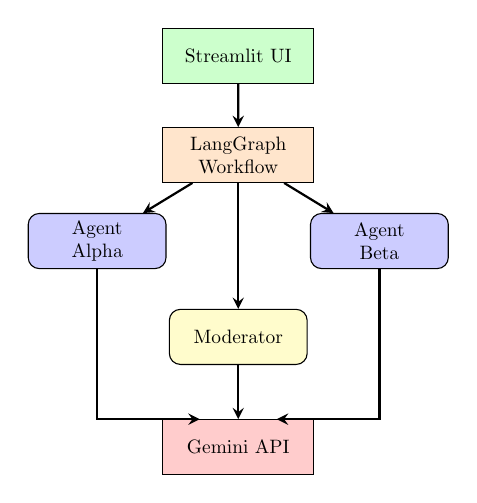
\begin{tikzpicture}[node distance=1.5cm, scale=0.7, transform shape]
            % UI Layer
            \node (streamlit) [process, fill=green!20, text width=2.5cm] {Streamlit UI};
            
            % Workflow Layer
            \node (langgraph) [process, below of=streamlit, yshift=-0.3cm, text width=2.5cm] {LangGraph\\Workflow};
            
            % Agent Layer
            \node (agent1) [agent, below left of=langgraph, xshift=-1.5cm, yshift=-0.5cm, text width=2cm] {Agent\\Alpha};
            \node (agent2) [agent, below right of=langgraph, xshift=1.5cm, yshift=-0.5cm, text width=2cm] {Agent\\Beta};
            \node (moderator) [agent, below of=langgraph, yshift=-1.8cm, fill=yellow!20, text width=2cm] {Moderator};
            
            % API Layer
            \node (gemini) [process, below of=moderator, yshift=-0.5cm, fill=red!20, text width=2.5cm] {Gemini API};
            
            % Arrows - with better positioning to avoid overlap
            \draw [arrow] (streamlit) -- (langgraph);
            \draw [arrow] (langgraph) -- (agent1);
            \draw [arrow] (langgraph) -- (agent2);
            \draw [arrow] (langgraph) -- (moderator);
            \draw [arrow] (agent1) |- ($(gemini.north) + (-0.7,0)$);
            \draw [arrow] (agent2) |- ($(gemini.north) + (0.7,0)$);
            \draw [arrow] (moderator) -- (gemini);
        \end{tikzpicture}
    \end{center}
    \vspace{0.3cm}
    \centering
    \footnotesize \textit{Figure: Multi-Layer System Architecture}
\end{frame}

% Slide 8: Technology Stack
\begin{frame}{Technology Stack \& Architecture}
    \begin{columns}
        \begin{column}{0.5\textwidth}
            \textbf{Core Technologies:}
            \begin{itemize}
                \item \textbf{Python 3.13}
                \begin{itemize}
                    \item Primary programming language
                    \item Rich AI/ML ecosystem
                \end{itemize}
                
                \item \textbf{Streamlit 1.51}
                \begin{itemize}
                    \item Web-based user interface
                    \item Real-time updates
                \end{itemize}
                
                \item \textbf{LangGraph 1.0.3}
                \begin{itemize}
                    \item Multi-agent orchestration
                    \item State management
                \end{itemize}
                
                \item \textbf{Google Gemini API}
                \begin{itemize}
                    \item LLM for argument generation
                    \item Natural language understanding
                \end{itemize}
            \end{itemize}
        \end{column}
        
        \begin{column}{0.5\textwidth}
            \textbf{Project Modules:}
            \begin{itemize}
                \item \textbf{Agents Module:}
                \begin{itemize}
                    \item Agent personality prompts
                    \item Response generation logic
                    \item Position assignment
                \end{itemize}
                
                \item \textbf{Graph Module:}
                \begin{itemize}
                    \item State definitions
                    \item Workflow implementation
                    \item Round management
                \end{itemize}
                
                \item \textbf{Main Application:}
                \begin{itemize}
                    \item User interface
                    \item Input handling
                    \item Results display
                \end{itemize}
            \end{itemize}
        \end{column}
    \end{columns}
\end{frame}

% Slide 9: Agent Design
\section{Implementation}
\begin{frame}{Dual-Agent Design Strategy}
    \begin{columns}
        \begin{column}{0.48\textwidth}
            \begin{block}{Agent Alpha}
                \footnotesize
                \textbf{Logical \& Analytical}
                
                \textbf{Characteristics:}
                \begin{itemize}
                    \scriptsize
                    \item Evidence-based arguments
                    \item Statistical references
                    \item Structured logic
                \end{itemize}
                
                \textbf{Strategy:}
                \begin{itemize}
                    \scriptsize
                    \item Factual data
                    \item Logical frameworks
                \end{itemize}
            \end{block}
        \end{column}
        
        \begin{column}{0.48\textwidth}
            \begin{block}{Agent Beta}
                \footnotesize
                \textbf{Passionate \& Persuasive}
                
                \textbf{Characteristics:}
                \begin{itemize}
                    \scriptsize
                    \item Emotional appeal
                    \item Real-world examples
                    \item Persuasive rhetoric
                \end{itemize}
                
                \textbf{Strategy:}
                \begin{itemize}
                    \scriptsize
                    \item Compelling stories
                    \item Human impact
                \end{itemize}
            \end{block}
        \end{column}
    \end{columns}
    
    \vspace{0.2cm}
    
    \begin{alertblock}{Response Constraints}
        \centering
        \footnotesize \textbf{Agents:} 200 words | \textbf{Moderator:} 250-300 words
    \end{alertblock}
\end{frame}

% Slide 10: LangGraph Workflow
\begin{frame}{LangGraph Workflow Implementation}
    \begin{columns}
        \begin{column}{0.48\textwidth}
            \textbf{Debate Flow Process:}
            \begin{enumerate}
                \small
                \item \textbf{Initialize State}
                \begin{itemize}
                    \footnotesize
                    \item Topic from user
                    \item Empty message list
                    \item Round counter = 0
                \end{itemize}
                
                \item \textbf{Agent 1 Response}
                \begin{itemize}
                    \footnotesize
                    \item Reads topic \& history
                    \item Generates argument
                \end{itemize}
                
                \item \textbf{Agent 2 Response}
                \begin{itemize}
                    \footnotesize
                    \item Reads opponent's argument
                    \item Generates counter-argument
                \end{itemize}
                
                \item \textbf{Round Check}
                \begin{itemize}
                    \footnotesize
                    \item If rounds remain $\rightarrow$ Repeat
                    \item If complete $\rightarrow$ Moderator
                \end{itemize}
            \end{enumerate}
        \end{column}
        
        \begin{column}{0.48\textwidth}
            \textbf{State Management:}
            \begin{itemize}
                \small
                \item \textbf{Topic Tracking}
                \begin{itemize}
                    \footnotesize
                    \item Maintains subject
                    \item Consistent context
                \end{itemize}
                
                \item \textbf{Message History}
                \begin{itemize}
                    \footnotesize
                    \item Stores all arguments
                    \item Enables rebuttals
                \end{itemize}
                
                \item \textbf{Round Counter}
                \begin{itemize}
                    \footnotesize
                    \item Tracks progress
                    \item Controls termination
                \end{itemize}
            \end{itemize}
            
            \vspace{0.2cm}
            
            \textbf{Final Step:}
            \begin{itemize}
                \small
                \item Moderator evaluates
                \item Declares winner
                \item Provides justification
            \end{itemize}
        \end{column}
    \end{columns}
\end{frame}

% Slide 11: Position Assignment Feature
\begin{frame}{Automatic Position Assignment}
    \begin{block}{Smart Topic Parsing}
        When users input topics with "vs", the system automatically assigns positions:
    \end{block}
    
    \vspace{0.3cm}
    
    \begin{columns}
        \begin{column}{0.5\textwidth}
            \textbf{How it Works:}
            \begin{itemize}
                \item Detects "vs" in topic
                \item Agent Alpha $\rightarrow$ Before "vs"
                \item Agent Beta $\rightarrow$ After "vs"
                \item Clear position indicators
            \end{itemize}
            
            \vspace{0.3cm}
            
            \textbf{Example Topics:}
            \begin{itemize}
                \item "Hardwork vs Talent"
                \item "AI vs Human Intelligence"
                \item "City vs Village Life"
            \end{itemize}
        \end{column}
        
        \begin{column}{0.5\textwidth}
            \begin{exampleblock}{Example: Hardwork vs Talent}
                \small
                \textbf{Agent Alpha:}\\
                Argues for \textcolor{blue}{Hardwork}
                
                \vspace{0.3cm}
                
                \textbf{Agent Beta:}\\
                Argues for \textcolor{purple}{Talent}
                
                \vspace{0.3cm}
                
                Each agent maintains their position throughout all rounds
            \end{exampleblock}
        \end{column}
    \end{columns}
\end{frame}

% Slide 12: Scoring & Rate Limiting
\begin{frame}{Key Features: Scoring \& Rate Limiting}
    \begin{columns}
        \begin{column}{0.48\textwidth}
            \begin{block}{Scoring System}
                \small
                \textbf{Evaluation Criteria:}
                \begin{itemize}
                    \footnotesize
                    \item Argument strength (30\%)
                    \item Evidence quality (25\%)
                    \item Logical coherence (20\%)
                    \item Rebuttal effectiveness (15\%)
                    \item Presentation clarity (10\%)
                \end{itemize}
                
                \vspace{0.2cm}
                
                \textbf{Outcome Categories:}
                \begin{itemize}
                    \footnotesize
                    \item Clear Winner: $>$ 3 points difference
                    \item Tie: $\leq$ 3 points difference
                \end{itemize}
            \end{block}
        \end{column}
        
        \begin{column}{0.48\textwidth}
            \begin{block}{Rate Limiting}
                \small
                \textbf{Challenge:}
                \begin{itemize}
                    \footnotesize
                    \item Free tier API limits
                    \item 429 errors without delays
                    \item Need for stable operation
                \end{itemize}
                
                \vspace{0.2cm}
                
                \textbf{Solution:}
                \begin{itemize}
                    \footnotesize
                    \item 2-second delays between calls
                    \item Prevents rate limit errors
                    \item Ensures stable operation
                    \item Smooth user experience
                \end{itemize}
            \end{block}
        \end{column}
    \end{columns}
\end{frame}

% Slide 13: User Interface
\begin{frame}{Streamlit User Interface}
    \textbf{UI Components:}
    \begin{itemize}
        \item \textbf{Topic Input:} Text field for debate subject
        \item \textbf{Round Selection:} Slider (1-5 rounds)
        \item \textbf{API Key Input:} Secure sidebar input
        \item \textbf{Position Display:} Shows each agent's arguing position
        \item \textbf{Real-time Streaming:} Live response generation
    \end{itemize}
    
    \vspace{0.5cm}
    
    \textbf{Color-Coded Display:}
    \begin{itemize}
        \item Agent Alpha - Blue boxes (Logical arguments)
        \item Agent Beta - Pink boxes (Passionate arguments)
        \item Moderator - Orange boxes (Final judgment)
    \end{itemize}
    
    \vspace{0.3cm}
    
    \begin{center}
        \colorbox{blue!10}{\textcolor{blue}{\textbf{Agent Alpha}}} \quad
        \colorbox{pink!30}{\textcolor{purple}{\textbf{Agent Beta}}} \quad
        \colorbox{orange!20}{\textcolor{orange!80!black}{\textbf{Moderator}}}
    \end{center}
\end{frame}

% Slide 14: Sample Results
\section{Results \& Evaluation}
\begin{frame}{Sample Debate Example}
    \begin{block}{Topic: "AI vs Human Intelligence"}
        \small
        \textbf{Agent Alpha (AI Intelligence) - Score: 42/50}\\
        "AI systems process vast datasets instantly, achieving superhuman performance in pattern recognition, chess mastery, and medical diagnosis..."
    \end{block}
    
    \vspace{0.2cm}
    
    \begin{block}{Agent Beta (Human Intelligence) - Score: 45/50}
        \small
        "Human intelligence encompasses creativity, emotional depth, and moral reasoning that no algorithm can replicate..."
    \end{block}
    
    \vspace{0.2cm}
    
    \begin{alertblock}{Moderator Verdict}
        \small
        \textbf{Winner: Agent Beta (Human Intelligence)}\\
        Tie with nuanced arguments. Beta's emphasis on irreplaceable human qualities slightly edges Alpha's technical capabilities.
    \end{alertblock}
\end{frame}

% Slide 15: Challenges & Solutions
\begin{frame}{Implementation Challenges \& Solutions}
    \begin{columns}
        \begin{column}{0.48\textwidth}
            \begin{block}{Technical Challenges}
                \small
                \textbf{1. Authentication Issues}
                \begin{itemize}
                    \footnotesize
                    \item LangChain auth errors
                    \item \textbf{Solution:} Direct Google SDK
                \end{itemize}
                
                \vspace{0.1cm}
                
                \textbf{2. Model Availability}
                \begin{itemize}
                    \footnotesize
                    \item Models not found
                    \item \textbf{Solution:} Used Gemini 2.0 Flash
                \end{itemize}
                
                \vspace{0.1cm}
                
                \textbf{3. Rate Limiting}
                \begin{itemize}
                    \footnotesize
                    \item 429 API errors
                    \item \textbf{Solution:} 2-second delays
                \end{itemize}
            \end{block}
        \end{column}
        
        \begin{column}{0.48\textwidth}
            \begin{block}{Design Challenges}
                \small
                \textbf{1. Response Length}
                \begin{itemize}
                    \footnotesize
                    \item Inconsistent token limits
                    \item \textbf{Solution:} 200-word limit
                \end{itemize}
                
                \vspace{0.1cm}
                
                \textbf{2. Position Assignment}
                \begin{itemize}
                    \footnotesize
                    \item Manual assignment tedious
                    \item \textbf{Solution:} Automated "vs" parsing
                \end{itemize}
                
                \vspace{0.1cm}
                
                \textbf{3. UI Readability}
                \begin{itemize}
                    \footnotesize
                    \item Poor color contrast
                    \item \textbf{Solution:} Dark text, light backgrounds
                \end{itemize}
            \end{block}
        \end{column}
    \end{columns}
\end{frame}

% Slide 16: Future Enhancements
\section{Future Work}
\begin{frame}{Future Work \& Enhancements}
    \begin{columns}[t]
        \begin{column}{0.48\textwidth}
            \textbf{Planned Features:}
            \begin{itemize}
                \small
                \item \textbf{Download Transcript}
                \begin{itemize}
                    \footnotesize
                    \item PDF export
                    \item TXT format
                \end{itemize}
                
                \item \textbf{Multi-Agent Extension}
                \begin{itemize}
                    \footnotesize
                    \item 3+ agents
                    \item Panel discussions
                \end{itemize}
                
                \item \textbf{Voice Integration}
                \begin{itemize}
                    \footnotesize
                    \item Text-to-speech
                    \item Audio debates
                \end{itemize}
            \end{itemize}
        \end{column}
        
        \begin{column}{0.48\textwidth}
            \textbf{Research Directions:}
            \begin{itemize}
                \small
                \item \textbf{Advanced Scoring}
                \begin{itemize}
                    \footnotesize
                    \item ML-based evaluation
                    \item Fact-checking
                \end{itemize}
                
                \item \textbf{User Participation}
                \begin{itemize}
                    \footnotesize
                    \item Human-AI debates
                    \item Audience voting
                \end{itemize}
                
                \item \textbf{Domain Specialization}
                \begin{itemize}
                    \footnotesize
                    \item Legal debates
                    \item Scientific discussions
                \end{itemize}
            \end{itemize}
        \end{column}
    \end{columns}
\end{frame}

% Slide 17: Conclusion
\section{Conclusion}
\begin{frame}{Conclusion}
    \begin{block}{Key Achievements}
        \footnotesize
        \begin{itemize}
            \item Successfully implemented dual-agent debate system
            \item Applied computational thinking principles
            \item Integrated Google Gemini API with LangGraph
            \item Created intuitive Streamlit interface
            \item Automated position assignment \& judgment
        \end{itemize}
    \end{block}
    
    \vspace{0.2cm}
    
    \begin{block}{Computational Thinking Application}
        \footnotesize
        Demonstrated all four CT pillars:
        \begin{itemize}
            \item \textbf{Decomposition:} Breaking debate into components
            \item \textbf{Pattern Recognition:} Argument structures
            \item \textbf{Abstraction:} State \& agent design
            \item \textbf{Algorithm Design:} Workflow implementation
        \end{itemize}
    \end{block}
\end{frame}

% Slide 18: References
\section{References}
\begin{frame}[allowframebreaks]{References}
    \footnotesize
    \begin{thebibliography}{99}
        \bibitem{wooldridge1995}
        Wooldridge, M., \& Jennings, N. R. (1995). 
        \textit{Intelligent agents: Theory and practice.} 
        The Knowledge Engineering Review, 10(2), 115-152.
        
        \bibitem{wing2006}
        Wing, J. M. (2006). 
        \textit{Computational thinking.} 
        Communications of the ACM, 49(3), 33-35.
        
        \bibitem{vaswani2017}
        Vaswani, A., et al. (2017). 
        \textit{Attention is all you need.} 
        Advances in Neural Information Processing Systems, 30.
        
        \bibitem{brown2020}
        Brown, T., et al. (2020). 
        \textit{Language models are few-shot learners.} 
        Advances in Neural Information Processing Systems, 33, 1877-1901.
        
        \bibitem{russell2020}
        Russell, S., \& Norvig, P. (2020). 
        \textit{Artificial Intelligence: A Modern Approach} (4th ed.). 
        Pearson.
        
        \bibitem{langgraph2024}
        LangChain. (2024). 
        \textit{LangGraph: Build stateful multi-agent applications.} 
        \url{https://langchain-ai.github.io/langgraph/}
        
        \bibitem{gemini2024}
        Google AI. (2024). 
        \textit{Gemini API Documentation.} 
        \url{https://ai.google.dev/docs}
        
        \bibitem{streamlit2024}
        Streamlit Inc. (2024). 
        \textit{Streamlit Documentation.} 
        \url{https://docs.streamlit.io/}
    \end{thebibliography}
\end{frame}

% Slide 19: Thank You
\begin{frame}
    \begin{center}
        \vspace{3cm}
        {\Huge \textbf{Thank You!}}
    \end{center}
\end{frame}

\end{document}
